\chapter{Project Structure}

I've created a custom implementation of Sagrada that allows a user to play interactively against 1-3 computer opponents using a graphical interface. 
Additionally, it can simulate games where multiple computer players (2-4) compete against each other, either interactively or through 
a command-line tournament. My implementation does not include the single player variant of the game where a player doesn't have any opponents
but tries to maximize the score with slightly different rules of the game.

\section{OS support}

I developed the game on Ubuntu, and it could potentially be ported to other operating systems such as Windows and other Linux distributions with relative ease, 
although I haven't attempted this. All the frameworks used in this project are cross-platform, enhancing the potential for easy adaptation.


\section{Language and 3rd party libraries}
For this project, the choice of the programming language primarily rested on the need for optimal performance and efficiency. 
I selected C++ as the programming language due to its reputation for producing highly performant code.

The following 3rd party libraries are used in the project:
\begin{enumerate}
    \item gtkmm - gtkmm \cite{gtkmm} is the official C++ interface for the popular GUI library GTK. GTK is widely used for creating graphical user interfaces 
    in applications that run on Linux, Windows, and macOS. I chose this library because it is easy to use, written in C++ and is cross-platform compatible.
    \item nlohmann\_json - an open-source library by Niels Lohmann \cite{nlohmann_json} for parsing JSON objects. It is mainly used for storing game configurations and for unit testing 
    \item argparse - an open-source library used for defining the command line interface \cite{argparse}
    \item googletest - an open-source library used for unit testing \cite{googletest}
\end{enumerate}

\section{Architecture}
The architecture of the system follows the Model-View-Controller (MVC) design pattern, because of its clear separation 
of concerns and scalability. In the MVC architecture, the model represents the application's data and game logic, the view 
handles the presentation layer, and the Controller manages user inputs and coordinates the communication between the model and the view components. 

This separation of concerns is important for many reasons. For instance, our system utilizes the model for different purposes, such as
running games and simulations using the GUI and running tournaments between AI players using the CLI.

\subsection{Model}
The model component is the backbone of the application, responsible for managing data and game logic. Concretely in Sagrada, this means:
\begin{enumerate}
    \item \textbf{Data management} - The model component in Sagrada holds the data about the game including the static data initialized 
    once at the beginning of the game (the different cards, dice, etc.), the current state of the game that is changing (round number, the player on move, etc.)
    and other data that is needed to perform the operations it defines (history of the game).
    \item \textbf{Game logic} - The game logic in Sagrada is represented by the actions that users of the Model component
    perform during the gameplay. These actions include collecting the possible moves, evaluating the sent moves for correctness
    or evaluating the current state of the game.

\end{enumerate}

The main class in the model component is \texttt{the Game class}. It has the following structure:


\begin{figure}[H]
    \caption{ Model structure UML diagram}
    \centerline{\mbox{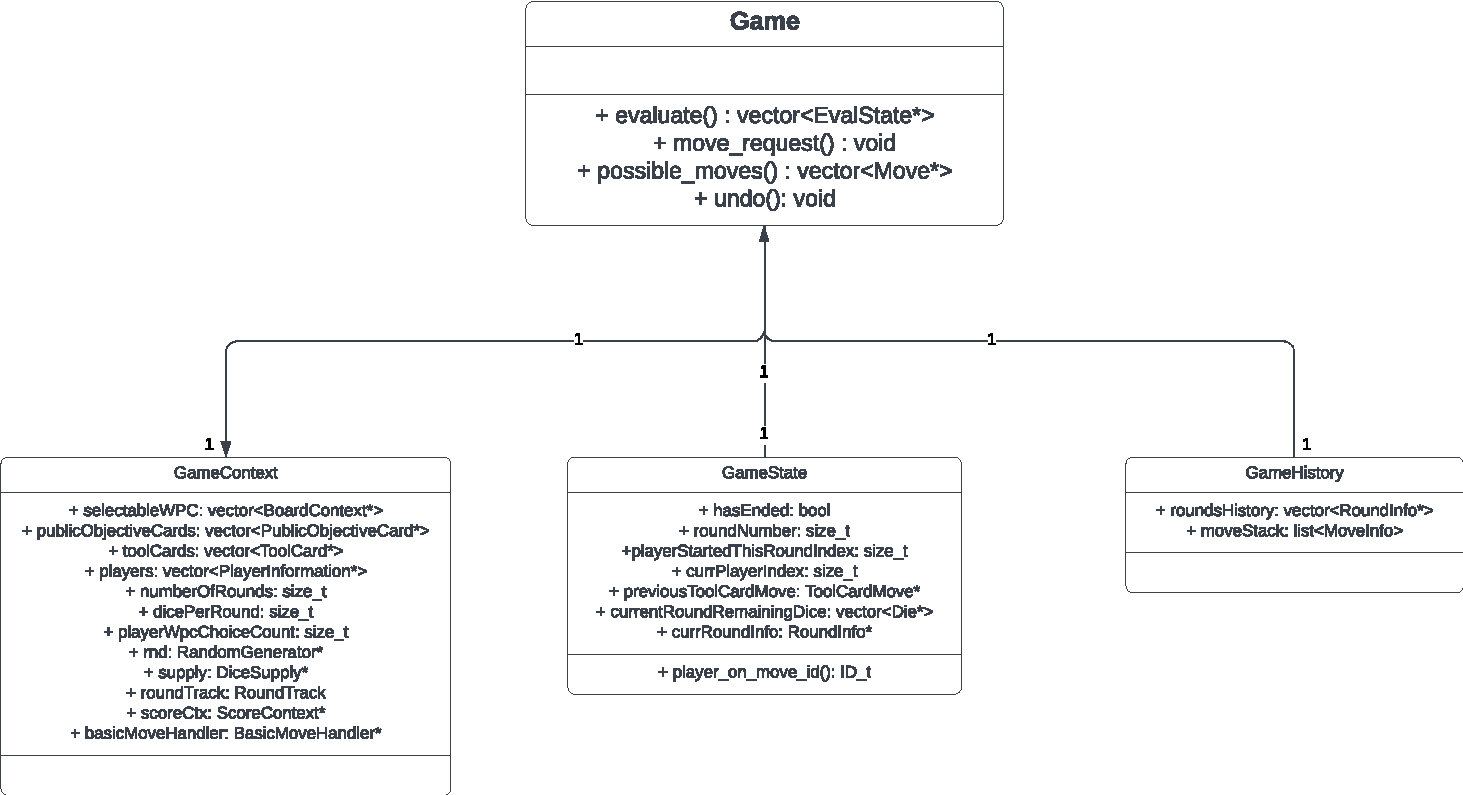
\includegraphics[width=166mm]{img/GameUML.pdf}}}
    \label{fig:Model_UML}
\end{figure}

The reason behind separating the data \texttt{the Game class} holds is connected to avoiding \texttt{the Game class} becoming a God object and following
design principles to achieve a higher factor of flexibility, maintainability and scalability.
\begin{description}
    \item[\texttt{GameContext}] This class represents the static data in \texttt{the Game class} class. Its components are once configured and 
    never changed after. The separation makes \texttt{the Game class} ' API smaller because creating these objects is the responsibility of the GameContextBuilder class.
    Also, it makes \texttt{the Game class} easily configurable by creating a \texttt{GameContext} instance and passing it to the constructor.
    \item[\texttt{GameState}] Dynamically changing data about the current state of \texttt{the Game class} . Having this class independently 
    also has reasons connected to making the API of \texttt{the Game class} smaller and bringing higher scalability.
    \item[\texttt{GameHistory}] Defining the Undo operation requires remembering the actions that lead to a given state of the class to be 
    able to reproduce past states. This class holds the data required for filling this functionality.
\end{description}

As illustrated on Figure \ref{fig:Model_UML} , \texttt{the Game class} has the following most important methods:

\begin{description}
    \item[\texttt{vector<Move*> possible\_moves()}] \label{principle:possible_moves} Returns the vector of all possible moves that are available for the current player at the current state. These
    moves include die-placing moves, Tool Card moves and a Pass move. First, if the previous move of the current player was a Tool Card move that consists
    of multiple sub-moves and there is a way to continue, the sub-moves that are the continuation of the previous sub-move are added. Second, if the player
    has enough favor tokens to use a Tool Card, the Tool Card moves are appended. After that, the die-placing moves are appended starting with dice on the lowest
    index in the \texttt{GameState::currentRoundsRemainingDice} container and the placing board indices are indexed starting from the upper left corner row-wise.
    Finally, the Pass move is added as the last move.
    \item[\texttt{void move\_request(move\_t move)}] Receives a move as an argument and checks whether it is a correct move or not. 
    \item[\texttt{void undo()}] Performs undo operation on the last move. This function is mainly used by AI agents like the minimax agent to produce better 
    performance than cloning every time \texttt{the Game object} a move is about to be evaluated.
    \item[\texttt{vector<EvalState*> evaluate()}] Evaluates the current game state for each player and returns a vector of \texttt{EvalState} objects. This function is called
    at the end of the game for final evaluation and by AI agents for evaluating the state after using given moves. 
\end{description}



\subsubsection{Moves} \label{subsec:Move_Implementation}
The different moves in the game are represented by derived classes from the Move class. Many Tool Cards define their
moves separately derived from ToolCardMove. There are two Tool Cards that consist of multiple sub-moves. The reason behind separating a single move
into multiple sub-moves is that these cards contain randomness meaning that a player chooses to use these Tool Cards, after the first sub-move the new random
value is revealed, and the second sub-move places the new die onto a field if possible. Concretely, these are the mentioned two Tool Cards:
\begin{enumerate}
\item \textbf{Flux Remover} - The first sub-move chooses a die from the Draft Pool to be swapped and swaps it with a die from the Bag. The second
sub-move chooses a value for the die from the Bag and places it onto a field if possible.
\item \textbf{Flux Brush} - The first sub-move chooses a die from the Draft Pool and re-rolls it. The second sub-move places the die onto a field.
\end{enumerate}

\subsection{View}

In this section, we're exploring the view component. I've chosen \texttt{gtkmm3-0} for its ease of use, cross-platform compatibility, and because it's written in C++.
The GUI is structured into pages. Each page in the GUI is equipped with widgets to fulfill specific functions. The two most important pages are the following:
\begin{itemize}
    \item \textbf{GamePlayingPage} - This page is a base class for \texttt{the LocalGamePlayingPage class} and \texttt{the SimulationGamePlayingPage class} 
    since these two pages have the same functionalities except for some user interactions. It displays all the elements of the game such as the boards 
    of the players or the current round's dice.
    \item \textbf{LocalGamePlayingPage} - This page is used when the user chooses to play against AI agents. This page has some specific functionalities 
    other than its base \texttt{class GamePlayingPage}.  These functionalities include selecting a die and placing it onto the player's board or using the Tool Cards.
    \item \textbf{SimulationGamePlayingPage} - This page is used for displaying simulations between AI agents. It is useful when during an experiment a game
    has strange results and we would like to check the steps each AI agent made leading to the odd result.
\end{itemize}



\subsection{Controller}

The Controller component serves as the intermediary between the model and the view components. It primarily handles user input, processes requests, 
and provides appropriate responses. Concretely in Sagrada, the Controllers manage the AI players and forward the human players' move requests in games with human players.

\texttt{The ControllerWithAIPlayer class} serves as a base class for the two concrete controllers.
It stores a reference to the game that is being played and stores the AI players by the corresponding player IDs. 

For playing games with human players, an instance of \texttt{the LocalPlayerController class} is used. This class is derived from 
\texttt{the ControllerWithAIPlayer class} making it able to play games with both human and AI Players. Additionally, it stores the IDs of all
human players providing easier handling for the view components. 

Games that are played between only AI players use an instance of \texttt{the OnlyAIPlayerController class} . This class is used mainly in the Tournament framework.  

\section{Tournament Framework}

Having the Tournament framework independent from the GUI makes experimenting faster and easier. This way it is possible to 
automatize running the different tournaments and processing their results by scripts. To run tournaments, run the 
\texttt{build/tournament} executable. It accepts the following arguments:

\begin{description}
    \item[-h] Displays help information. \\
    \item[-v] Prints the results to the standard output game-by-game. This option is turned off by default.\\
    \item[-s] The starting seed of the tournament i.e. the seed of game 1. The default value is 779. \\
    \item[-n] The number of games in the tournament. There is no default value for this option and it is required to specify one.\\
    \item[-d] Makes the games in the tournament deterministic i.e. all the information is available for all the agents including dice in the upcoming rounds and other players' Private Objective Cards. This option is turned off by default.\\
    \item[-p] The agents that will play against each other in the tournament. This option accepts 2-4 parameters and has no default configuration but it is required to be defined.
    \begin{description}
        \item[random] - An agent choosing a random move
        \item[first] - An agent choosing the first possible move
        \item[rules-based] - An agent with rules-based strategy. \\Example config: rules-based-strategy=only\_dtfm
          \begin{description}
            \item[strategy] Choose a strategy for the player. The two possible options are \textbf{only\_dtfm} and \textbf{all\_moves}
          \end{description}
        \item[minimax] - Minimax agent. \\ Example config: minimax-depth=3,worlds=8,config\_file=config.json
          \begin{description}
            \item[depth] Sets the depth for the minimax search.
            \item[worlds] Sets the determinizing world count.
            \item[config\_file] Sets a config file with heuristic constants.
          \end{description}
        \item[mcts] - Monte Carlo Tree Search agent. \\Example config: mcts-it=120,expl=0.7,worlds=6,playout=random
          \begin{description}
            \item[it] Sets the iteration count for the algorithm.
            \item[worlds] Sets the determinizing world count.
            \item[expl] Sets the exploration constant for the algorithm.
            \item[playout] Sets the playout strategy for the simulation step of the algorithm.
          \end{description} 
      \end{description}
    
    \item[-mode] The mode of the game. Allows the users to run tournaments with a custom configuration. The default value is ``default''.\\
    \item[-b] Runs all the permutations of players in a game using a given seed. This option is turned off by default.\\
    \item[-csv] An option to save the results of the game into a directory of CSV files. The parameter is the name of the directory. This option is turned off by default.\\
    \item[-ms] An option to save information about the branching factor of each player. This option is turned off by default.\\
    \item[-gi] An option to save additional information for each game such as the Tool Cards or the Public Objective Cards used in the game. This option is turned off by default.\\ 
\end{description}
  
An example of running a tournament of 100 games using 800 as the starting seed between a minimax agent and a rules-based agent:
\begin{verbatim}
$ build/tournament -n 100 -p rules-based-strategy=only_dtfm \ 
minimax-depth=4,worlds=4 -s 800 -v
\end{verbatim}
  

When the tournament ends, the framework prints statistics about the game and the players either to the standard output or to the specified CSV files. The statistics include
the number of games won by each player, the average time it took for each player to make a move and the Wilson confidence interval for the tournament-winning player.

A random seed is a number used to initialize a pseudorandom number generator. By setting this seed, the starting point for a sequence of pseudorandom numbers
is determined. This means that changing this random seed for a game results in another game configuration and that way another gameplay. On the other hand,
this also means that using the same seed multiple times produces the same output. The tournament framework uses the random seed received from the command-line
and increases it by one after every game. This means that if the first game used the random seed 779, the second one will use 780 and so on.

There is an option to simulate games played between AI agents using the GUI. This comes in handy if some games produce an interesting outcome in the tournament and the user
would like to check the choices of the AI agents one by one. The CLI is designed to make this task as user-friendly as possible. To simulate a game
that was run in the tournament using the following command:
\begin{verbatim}
$ build/tournament -n 100 -p rules-based-strategy=only_dtfm \
minimax-depth=4,worlds=4 -s 800 -v
\end{verbatim}

run the following command:

\begin{verbatim}
$ build/sagrada simulation -p rules-based-strategy=only_dtfm \
minimax-depth=4,worlds=4 -s 800 -v
\end{verbatim}
  

% \section{Data Processing Scripts}

% This section describes how the given scripts work with the results of the tournaments. The scripts are written in Python
% and I am using different tools to visualize the results of given experiments such as matplotlib or prettytable. The overall
% structure of the data flow is illustrated in the following diagram:


% \begin{figure}[H]
%     \caption{ CSV data flow UML diagram}
%     \centerline{\mbox{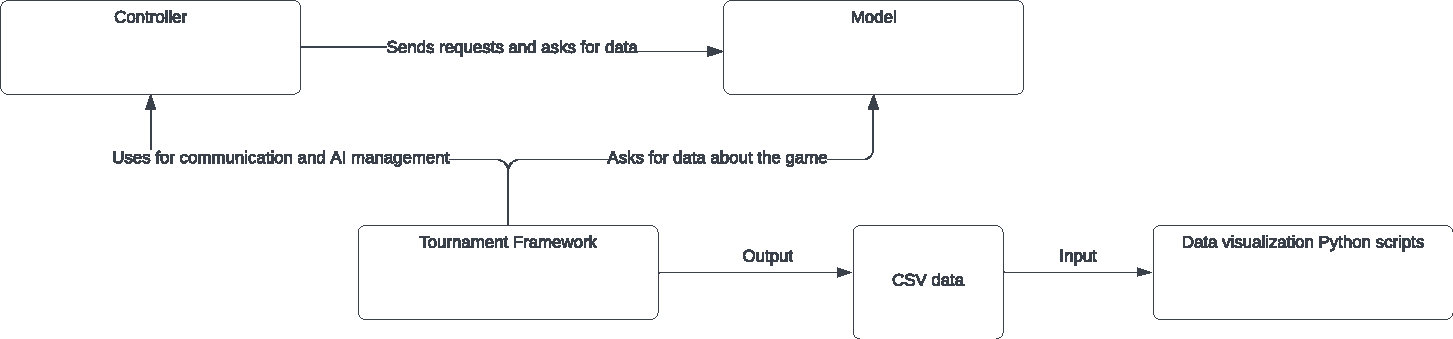
\includegraphics[width=166mm]{img/CSVDataFlow.pdf}}}
%     \label{fig:example}
% \end{figure}

